%-------------------------
% Beamer
% Author : Tansheng Zhu
% Based on: https://github.com/sjtug/SJTUBeamer/blob/main/main.tex
% License : CC-BY-SA 4.0
%------------------------

\makeatletter
\def\input@path{{styles/}}
\makeatother

\documentclass[aspectratio=169]{beamer}
\usepackage[UTF8, scheme=plain, punct=plain, zihao=false]{ctex}

\usepackage[ruled, linesnumbered]{algorithm2e}
\usepackage{fontawesome}
\usepackage{longtable}
\usepackage{makecell}
\usepackage[mathscr]{eucal}
\usepackage{multicol}
\usepackage{siunitx} % \SI{}{}
\usepackage{bm}
\usepackage{bbm} % \mathbbm{1}
\usepackage[noabbrev,capitalize]{cleveref}

\mode<presentation>

\usepackage[
    backend=bibtex,
    citestyle=authoryear-comp,
    bibstyle=numeric,
    maxbibnames=9,maxcitenames=2,uniquelist=false,
]{biblatex}
\addbibresource{references.bib}

% -------------------- GLOBAL OPTIONS --------------------
\usetheme[
    zts1, % [maxplus|max|min] 主要主题, [zts1|zts2] 自定义
    blue, % [red|blue] 主色调
    light, % [dark|light] 暗色/亮色模式
    topright, % [topright|bottomright] 徽标位置
    infolines, % [miniframes|infolines|sidebar|default|smoothbars|split|shadow|tree|smoothtree] 外样式
]{sjtubeamer}

\AtBeginSection[]{
    \begin{frame}
        % 普通目录
        % \frametitle{Table of Contents}
        % \tableofcontents[sectionstyle=show/shaded,subsectionstyle=show/show/hide]

        % 主题节页
        \sectionpage
    \end{frame}
}


% -------------------- CUSTOM COMMANDS --------------------
\newcommand{\hlt}[1]{\textcolor{red}{\bf #1}}

\newcommand{\dif}{\mathop{}\!\mathrm{d}}
\newcommand{\set}[1]{\left\{#1\right\}}
\newcommand{\diag}[1]{\mathrm{diag}\left\{#1\right\}}
\newcommand{\limit}[1]{\lim\limits_{#1}}
\newcommand{\limitsup}[1]{\limsup\limits_{#1}}
\newcommand{\limitinf}[1]{\liminf\limits_{#1}}
\newcommand{\trace}[1]{\mathrm{tr}\left(#1\right)}
\newcommand{\ts}{\mathsf{T}}

\DeclareMathOperator{\E}{\mathbbm{E}}
\DeclareMathOperator{\Var}{\mathbbm{V}\mathrm{ar}}
\DeclareMathOperator{\Cov}{\mathbbm{C}\mathrm{ov}}

\DeclareMathOperator*{\argmin}{argmin}
\DeclareMathOperator*{\argmax}{argmax}


% -------------------- TITLE PAGE --------------------
\title{SJTU Beamer Template}
\subtitle{Beamer Template}
\author[Tansheng Zhu]{
    Tansheng Zhu
    \footnotetext{\href{mailto:tsuthansing@sjtu.edu.cn}{tsuthansing@sjtu.edu.cn}}
}
\institute[SJTU]{
    Zhiyuan College \\
    Shanghai Jiao Tong University
}
\date{\today}

% SJTU: zts1+blue
\logo{\zhlogo}

% CUHK: zts2+red
% \logo{
\includegraphics{vi/cuhk-dlogo.png}}
% \titlegraphic{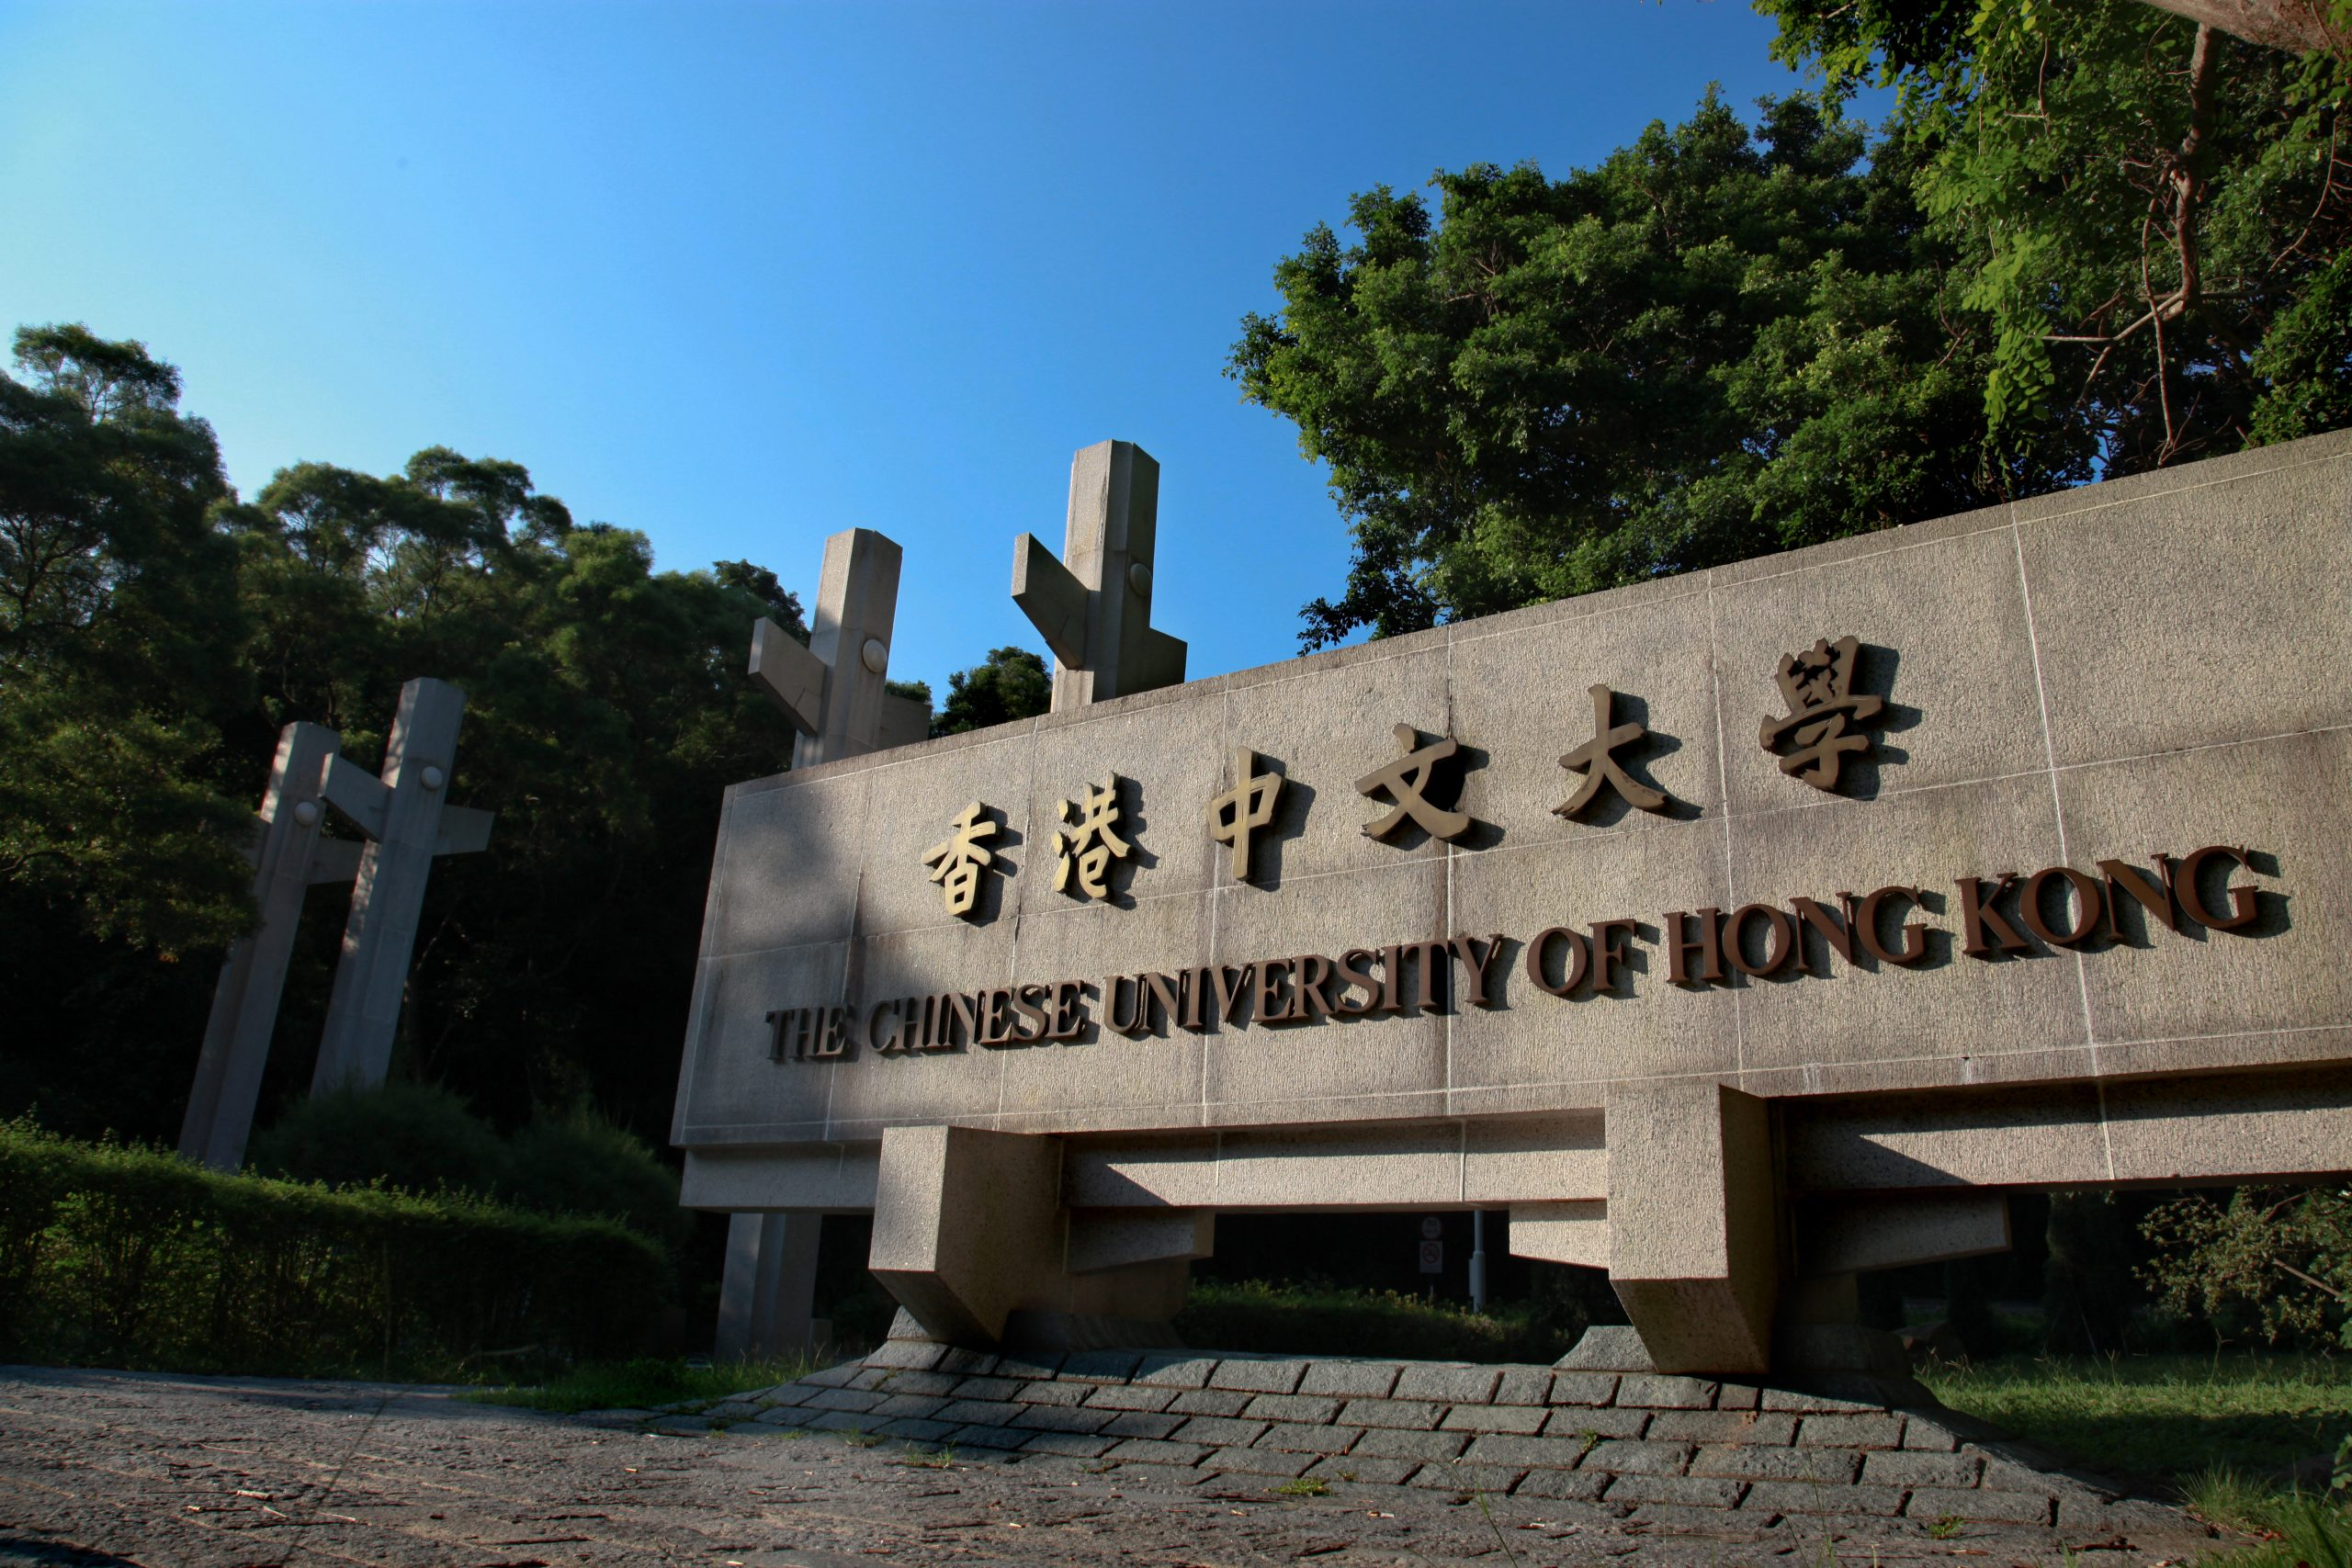
\includegraphics{vi/cuhk-cuhkphoto.jpg}}


% -------------------- START OF DOCUMENT --------------------
\begin{document}

% 标题页
\renewcommand{\thefootnote}{\faEnvelopeO}
\maketitle
\renewcommand{\thefootnote}{\arabic{footnote}}


% 目录页
% \begin{frame}[label=toc]
%     \frametitle{Table of Contents}

%     % 单栏目录
%     % \tableofcontents

%     % 双栏目录
%     % \begin{multicols}{2}
%     %     \tableofcontents
%     % \end{multicols}
% \end{frame}



\section{问题背景}

\begin{frame}
    \frametitle{title}
    \framesubtitle{subtitle}

    \begin{columns}[T]
        \begin{column}{0.3\textwidth}
            \begin{block}{盒子}
                ...
            \end{block}
        \end{column}
        
        \begin{column}{0.7\textwidth}
            \begin{alertblock}{注意}
                ...
            \end{alertblock}
            \begin{exampleblock}{示例}
                ...
            \end{exampleblock}
        \end{column}
    \end{columns}
\end{frame}



\section{主要内容}

\begin{frame}
    \frametitle{title}
    \framesubtitle{subtitle}
    
    \begin{itemize}
        \item Random Search: 采样点服从定义域上的均匀分布.
        \item GP-UCB: 由于迭代次数较少, 设置探索--利用权衡超参数 $\beta_t^{1/2}$ 为常数.
        \begin{equation*}
            \bm{x}_{t+1} = \argmax_{\bm{x} \in \mathcal{D}} \left( \mu_t(\bm{x}) + \beta_t^{1/2} \sigma_t(\bm{x}) \right),
        \end{equation*}
        \item KR-UCB: 基于离散UCB1公式的采集函数, 其中 $h_t \propto t^{-1/(d+4)}$ (Scott's rule).
        \begin{align*}
            \bm{x}_{t+1} &= \argmax_{\bm{x} \in \mathcal{D}} \left( W_t^{-1}(\bm{x}) \mathbbm{1}_{\set{\| \bm{x} - \bm{x}^{(t)} \|_2 \le \mathcal{T}}}(\bm{x}) \right), 
            \\
            \bm{x}^{(t)} &= \argmax_{\bm{x} \in \bm{D}_t} \left( m_t(\bm{x}) + C \sqrt{\dfrac{\ln \sum_{\bm{y} \in \bm{D}_t} W_t(\bm{y})}{W_t(\bm{x})}} \right).
        \end{align*}
    \end{itemize}
\end{frame}


\begin{frame}
    \frametitle{title}
    \framesubtitle{subtitle}

    \begin{algorithm}[H]
        \caption{Monte Carlo Tree Search}\label{alg:MCTS}
        \SetKwFunction{MctsSearch}{MctsSearch}
        \SetKwFunction{TreePolicy}{TreePolicy}
        \SetKwFunction{RolloutPolicy}{RolloutPolicy}
        \SetKwFunction{Update}{Update}
        \SetKwFunction{BestChild}{BestChild}
        \SetKwProg{fn}{Function}{:}{}
    
        \fn{\MctsSearch{$s_0$}}{
            Create root node $v_0$ with initial state $s_0$ \;
            \While{within computational budget}{
                $v_l \leftarrow$ \TreePolicy{$v_0$} \;
                $Q \leftarrow$ \RolloutPolicy{$s(v_l)$} \;
                \Update{$v_l$, $Q$} \; 
            }
            \Return{$a($\BestChild{$v_0$}$)$} \;
            \BlankLine
        }
        \textbf{end}
    \end{algorithm}
    \cref{alg:MCTS}, \cite{miktex}
\end{frame}



\section{参考文献}

\begin{frame}[allowframebreaks]    
    \nocite{*} % 如果全文无引用,但想排印所有条目    
    \printbibliography[heading=none] % 排印引用条目
\end{frame}



% -------------------- END OF DOCUMENT --------------------
\renewcommand{\thefootnote}{\faEnvelopeO} % 邮箱符号
\makebottom

\end{document}
